% !Mode:: "TeX:UTF-8"

\chapter{Foreign Language Material}

\section{The Information of The Foreign Language Material}
V. Demir and A. Z. Elsherbeni, "Programming finite-difference time-domain for graphics processor units using compute unified device architecture," 2010 IEEE Antennas and Propagation Society International Symposium, Toronto, ON, 2010, pp. 1-4. doi: 10.1109/APS.2010.5562117

\section{The Original of The Foreign Language Material}

\begin{figure}[h]
\centering
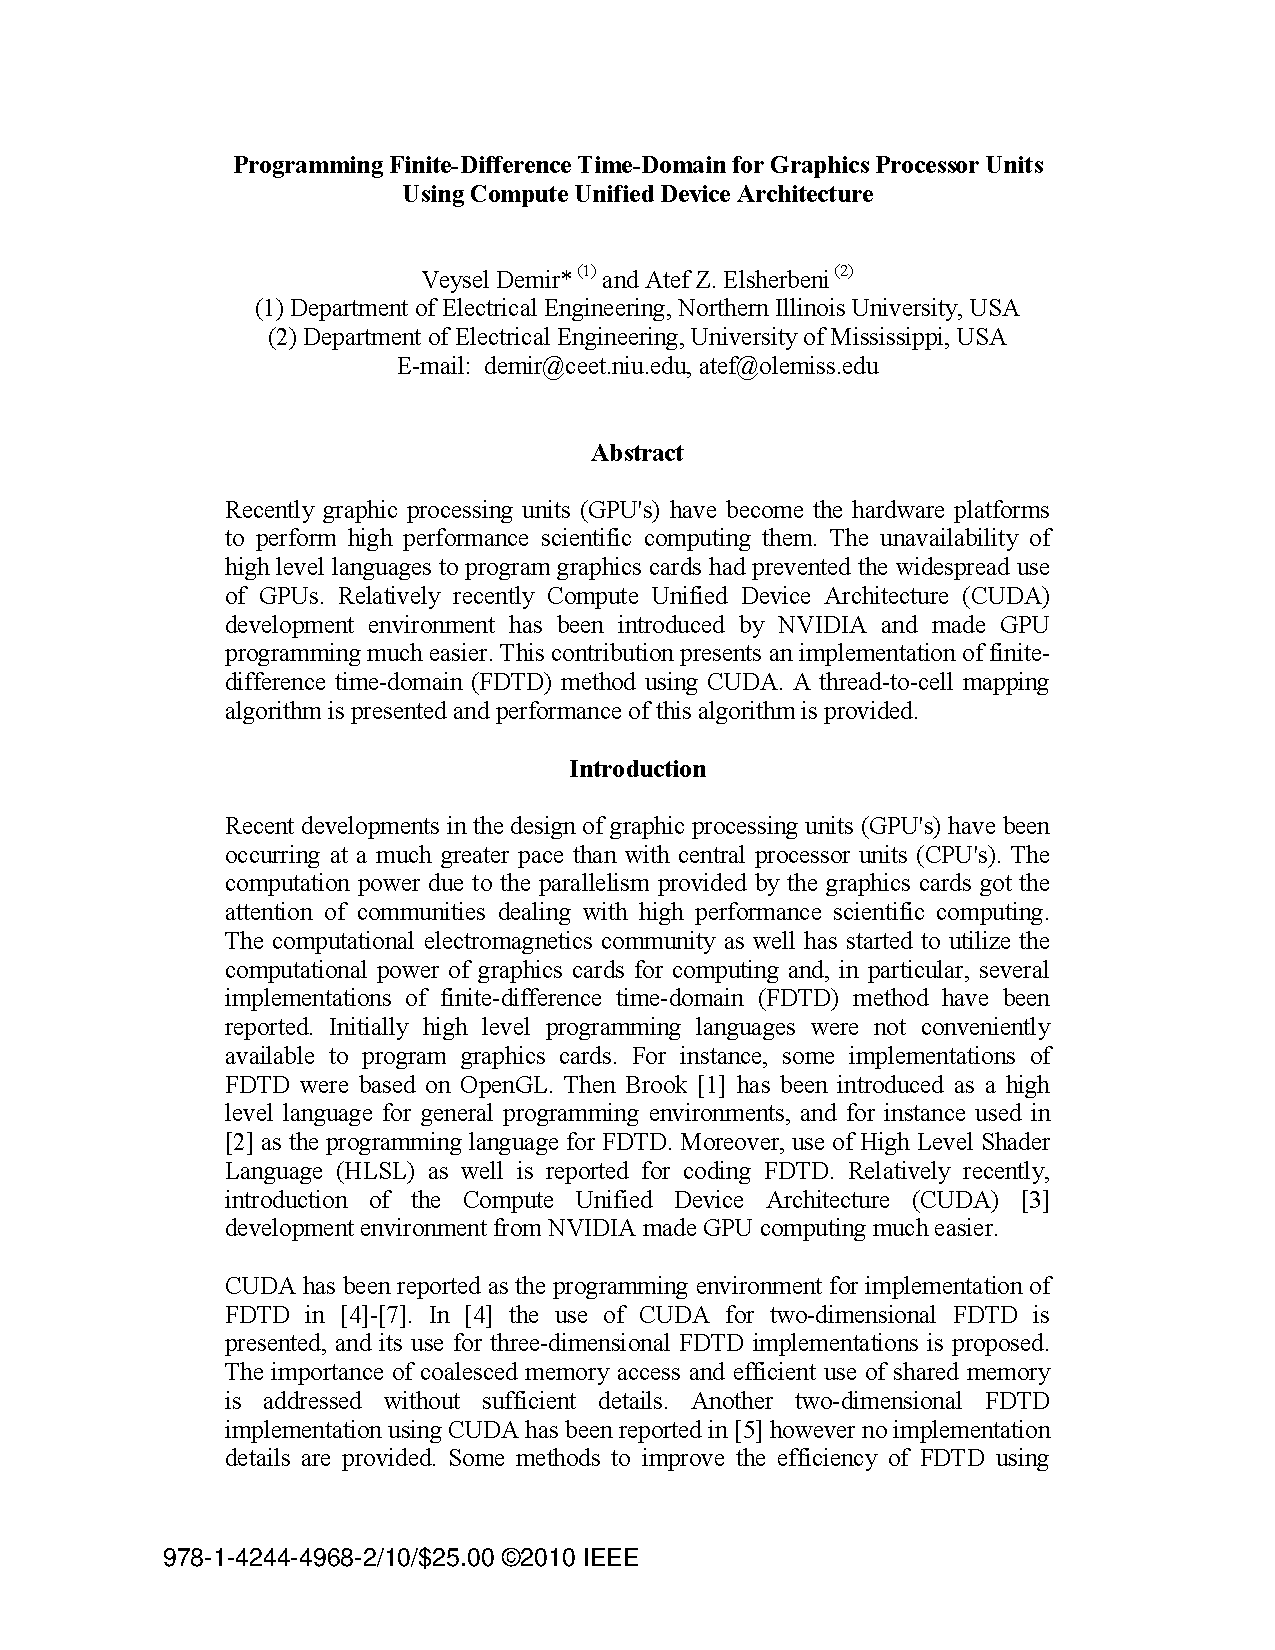
\includegraphics[width=1\linewidth,height=0.8\textheight]{../pics/p01}
\caption{The first page of the original}
\label{fig:p01}
\end{figure}

\begin{figure}[h]
	\centering
	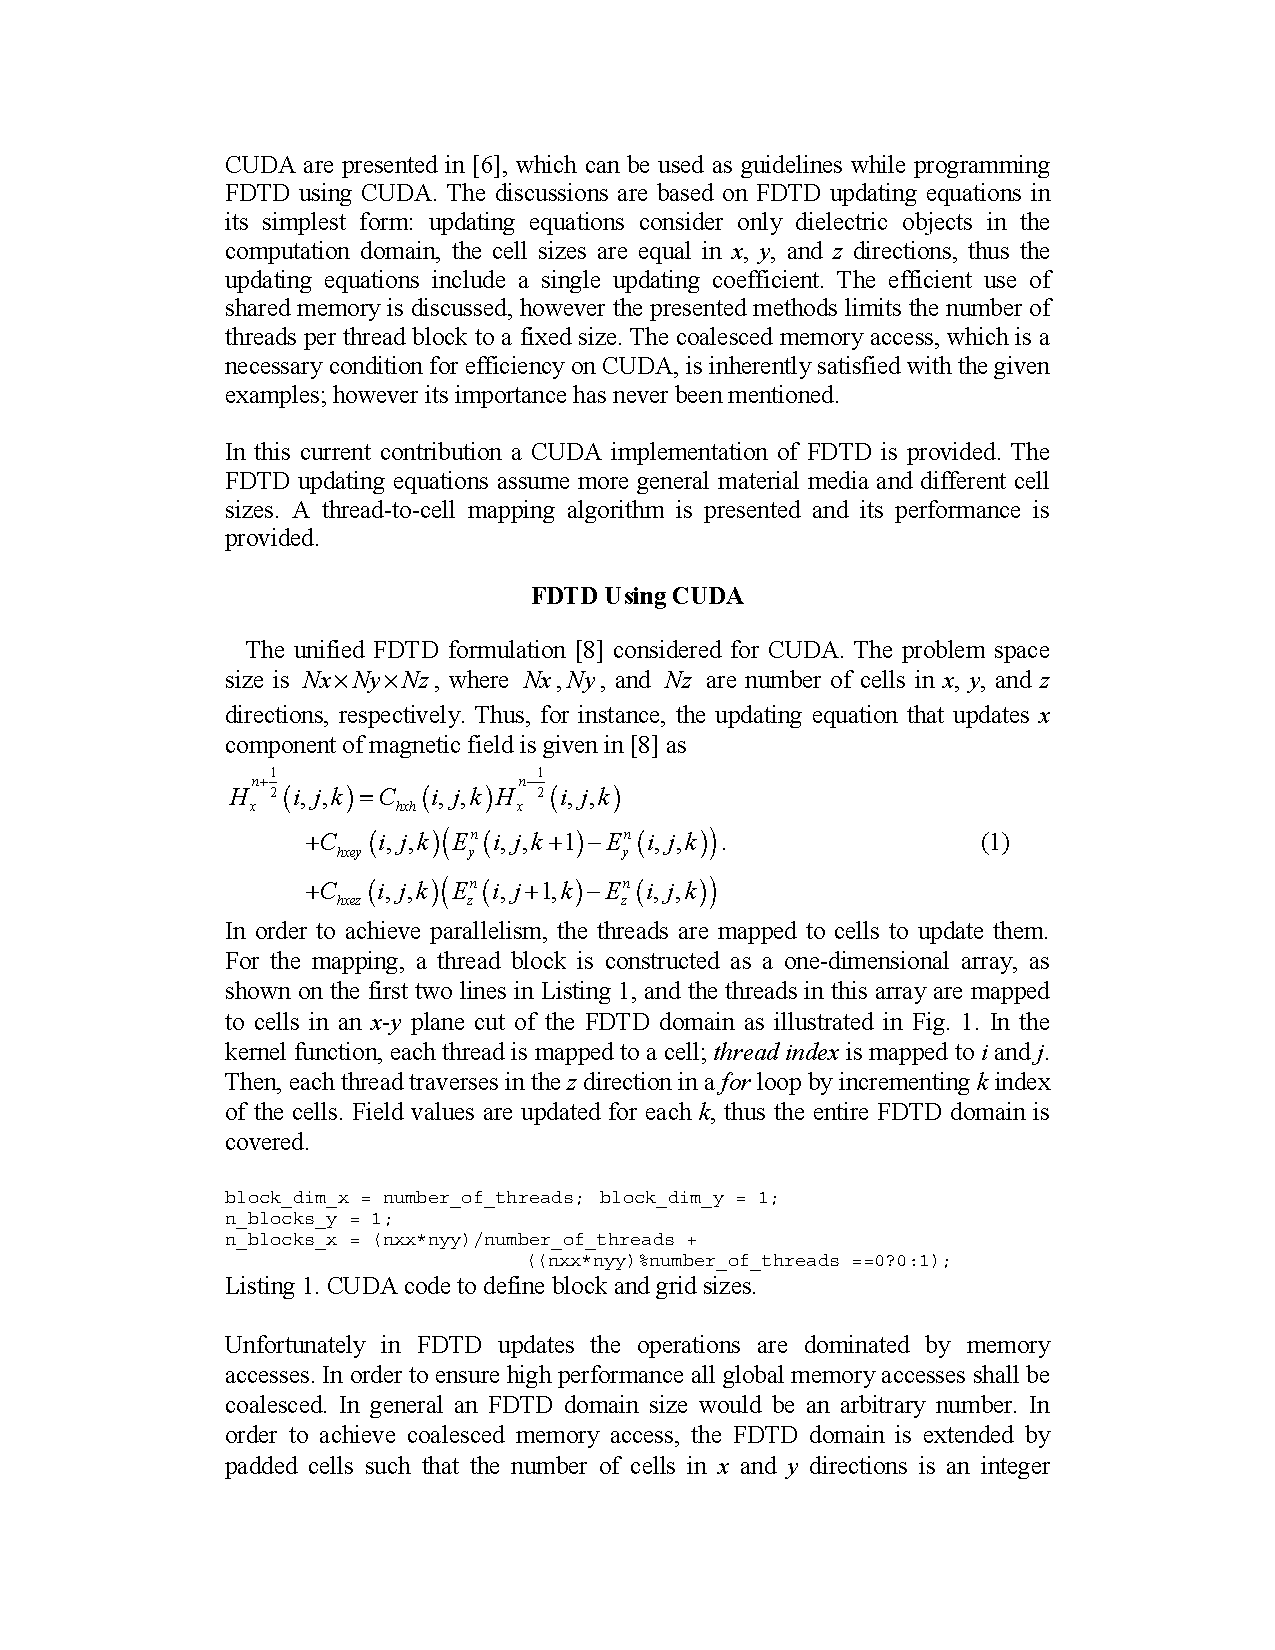
\includegraphics[width=1\linewidth]{../pics/p02}
	\caption{The second page of the original}
	\label{fig:p02}
\end{figure}

\begin{figure}[h]
	\centering
	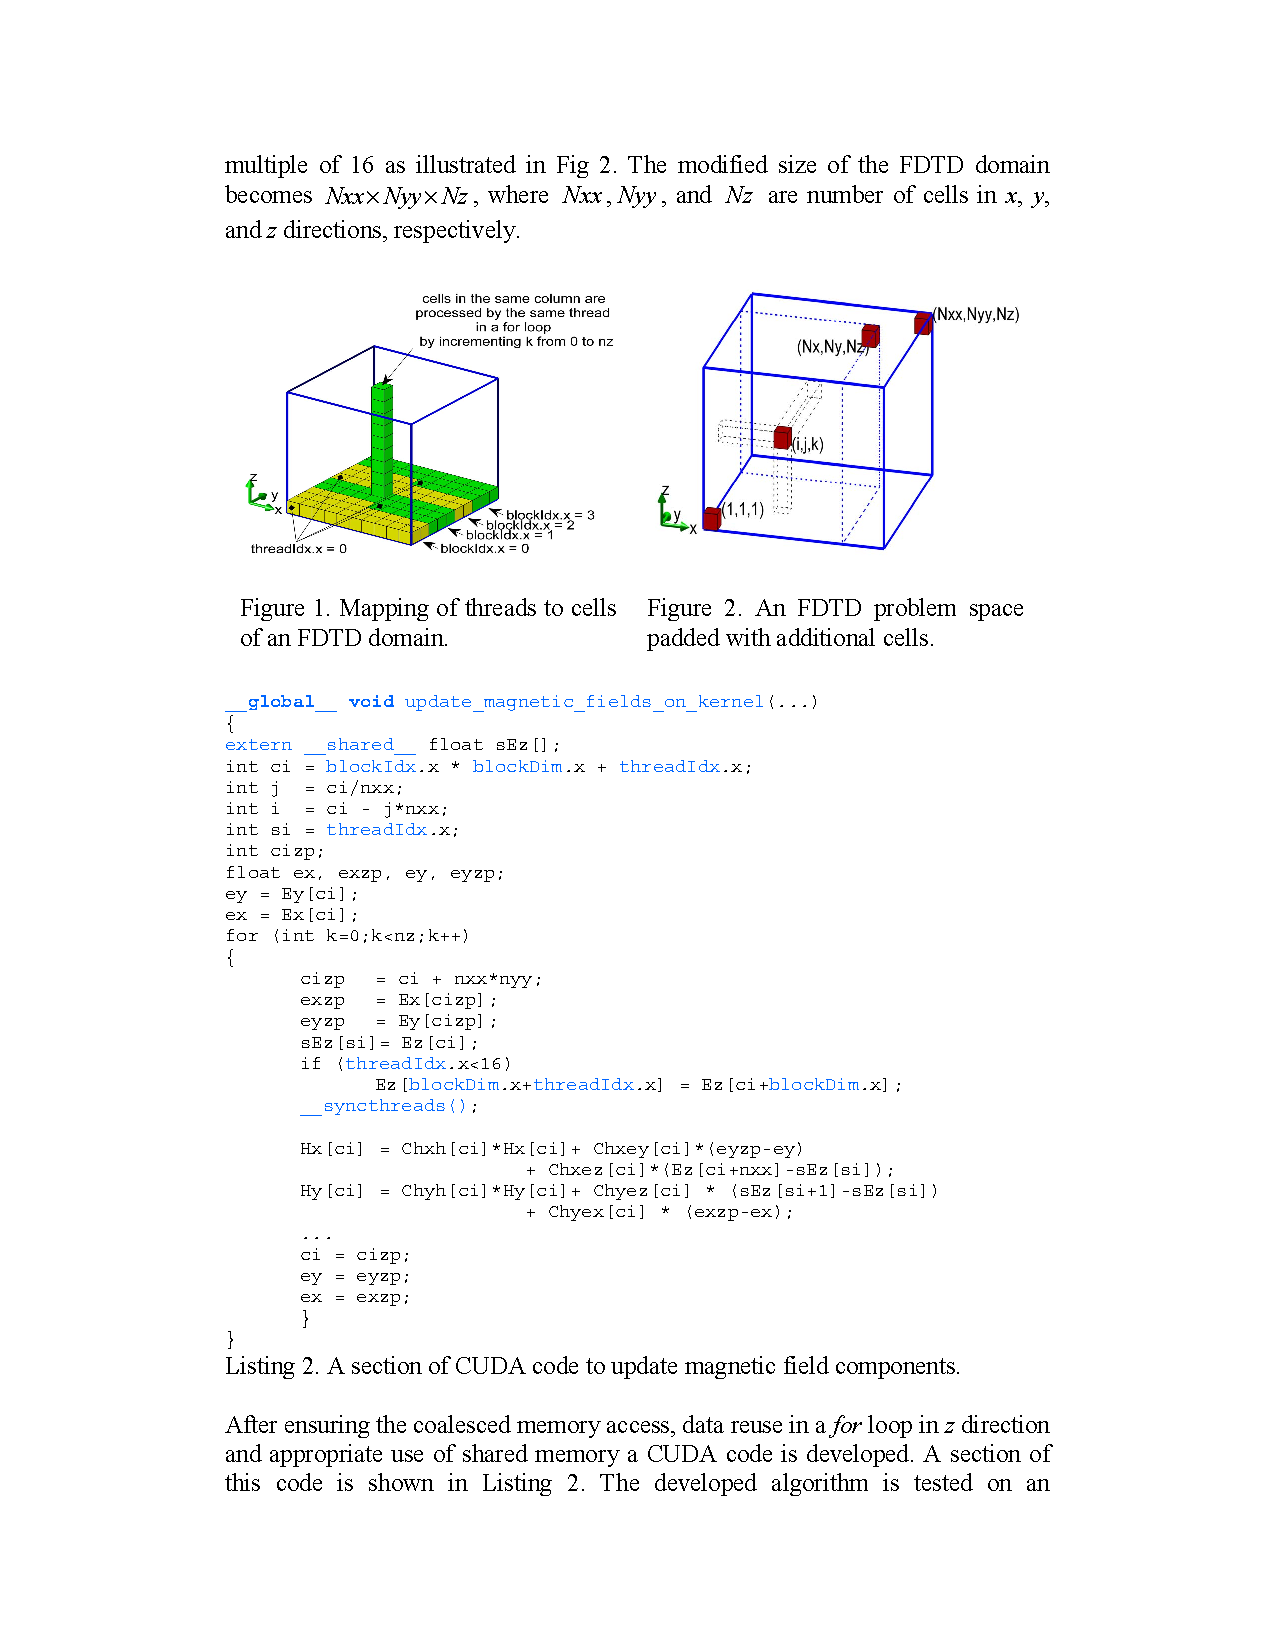
\includegraphics[width=1\linewidth]{../pics/p03}
	\caption{The third page of the original}
	\label{fig:p03}
\end{figure}

\begin{figure}[h]
	\centering
	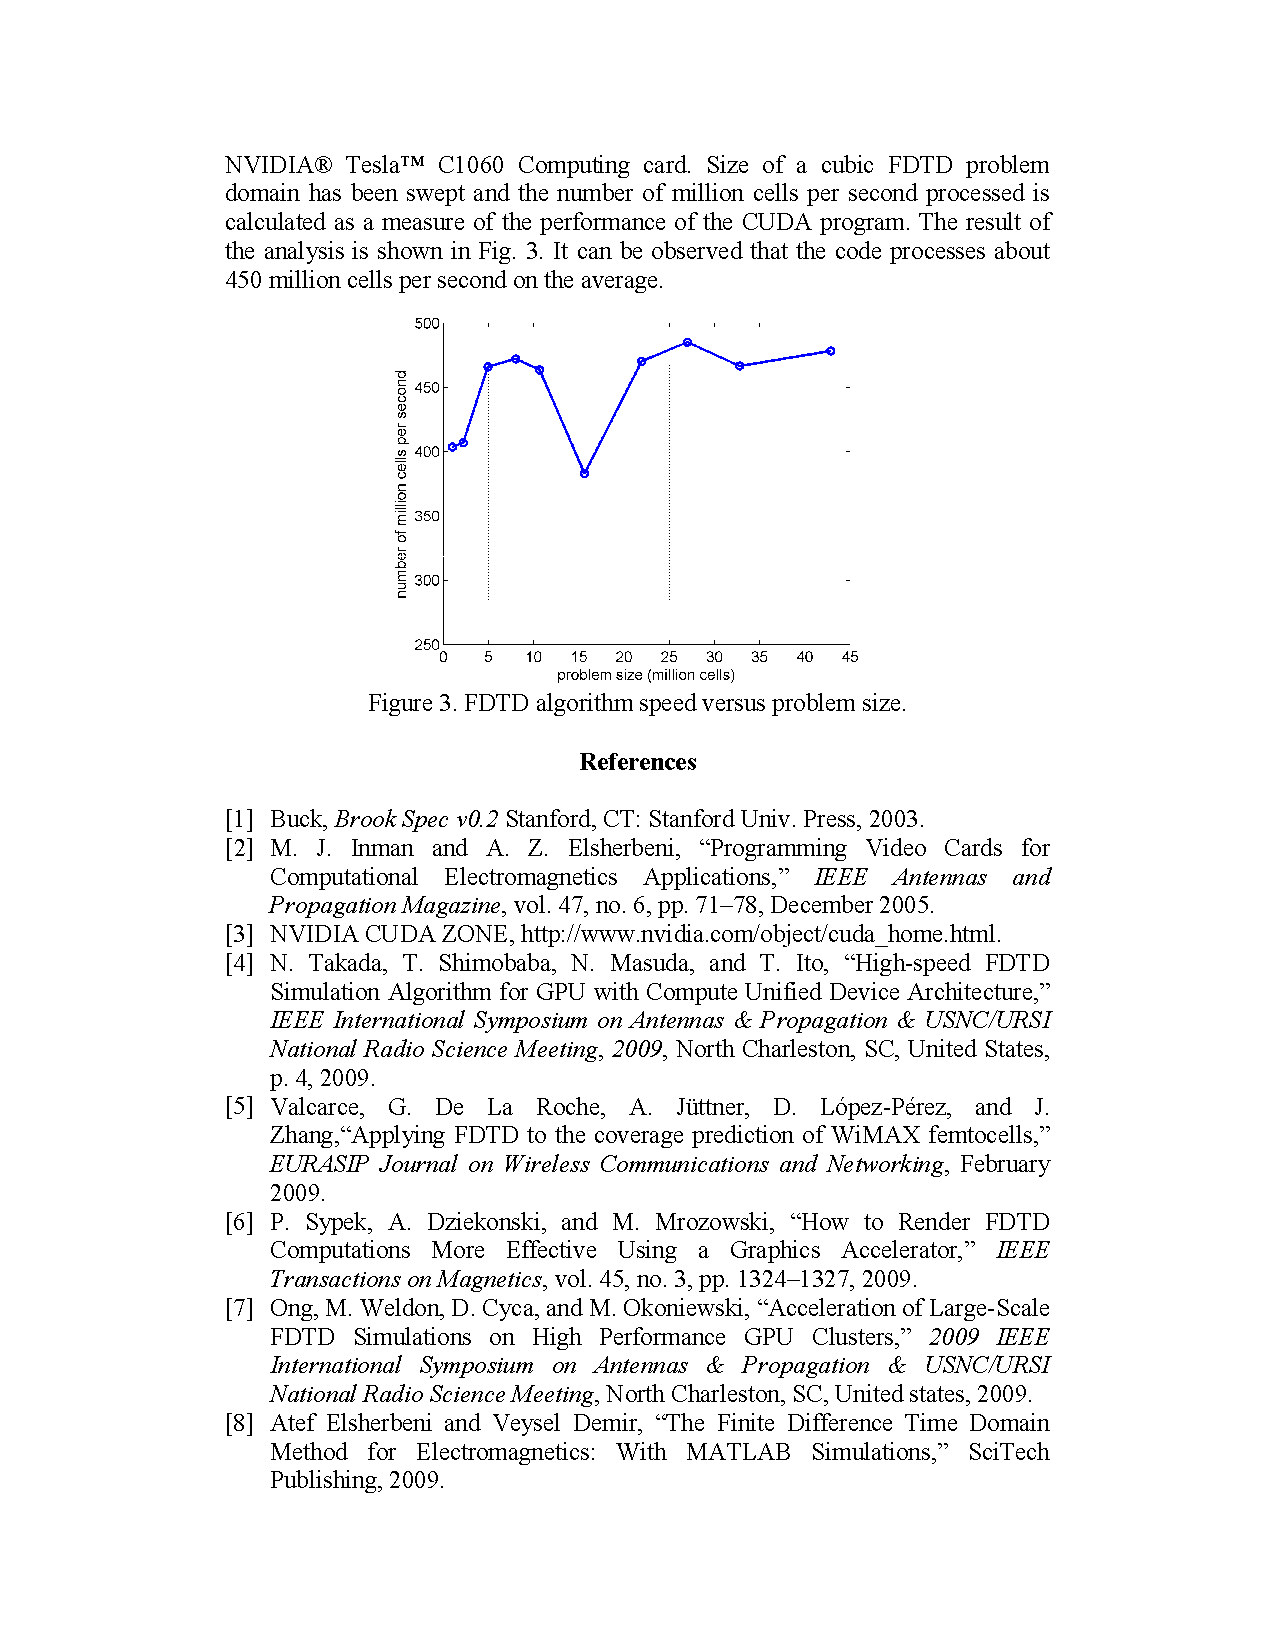
\includegraphics[width=1\linewidth]{../pics/p04}
	\caption{The fourth page of the original}
	\label{fig:p04}
\end{figure}